

\documentclass[12pt, a4paper]{article}

\usepackage{array}
\usepackage{float} 
\usepackage[a4paper, total={15cm , 26cm}]{geometry}
\usepackage{graphics}
\usepackage{hyperref}
\usepackage{karnaugh-map}

\graphicspath{{./images/}}

\title{\LaTeX \ Basics Session 2 \\ Sample Document 1}
\author{Written by: Me :)}
\date{\today}

\begin{document}
  \maketitle
  \section{Introduction}
      In this sample document will contain different types of fonts that can be used in \LaTeX documents, as well as different kinds of stuff you can add, ranging from images to tables and the like.

  \section{Images}
      Here you can add images to your document with ease with a couple of commands:

      \begin{figure}[H]
          \centering
          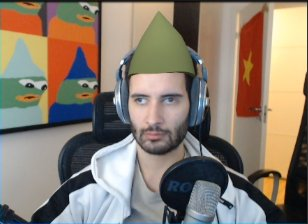
\includegraphics[scale = 0.7]{FeelsDankMan.jpg}
          \caption{This is a caption of a Swedish Streamer. FeelsDankMan}
      \end{figure} 

  \newpage
  \section{Tables}

      Here, you can even create your own tables:

      \begin{table}[H]
          \centering
          \begin{tabular}{|| m{2em} | m{2em} | m{2em} | m{2em} ||}
            \hline
            A &B &C &f \\ \hline \hline 
            0 &0 &0 &0 \\ \hline
            0 &0 &1 &1 \\ \hline
            0 &1 &0 &0 \\ \hline
            0 &1 &1 &1 \\ \hline
            1 &0 &0 &1 \\ \hline
            1 &0 &1 &0 \\ \hline
            1 &1 &0 &1 \\ \hline
            1 &1 &1 &0 \\ \hline
          \end{tabular}
          \caption{Another caption but for this truth table}
      \end{table}

  \section{Karnaugh Maps}
      You know there are custom packages available from CTAN right? Here's one you can use for karnaugh maps:
      
      \begin{figure}[H]
        \centering
        \begin{karnaugh-map}[4][4][1][$AB$][$CD$]
          \minterms{1, 3, 7, 8, 10}
          \maxterms{2, 4, 9, 11, 13, 14, 15}
          \terms{0, 5 , 6, 12}{X}

          \implicant{4, 12}
          \implicant[2, 10]
        \end{karnaugh-map}
      \end{figure}  

  \section{Equations}


\end{document}  